\documentclass{standalone}
\usepackage{tikz,amsmath}
\usetikzlibrary{quotes,angles}
\begin{document}
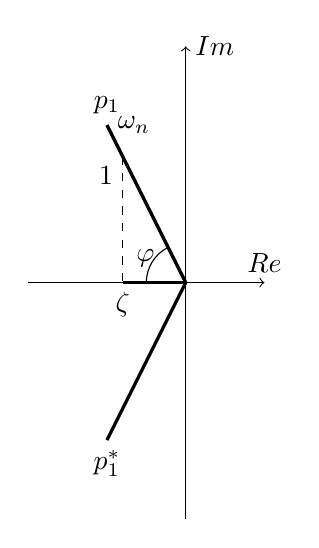
\begin{tikzpicture}[scale=2]
    \coordinate(O)at(0,0);
    \draw[->](-1,0)coordinate(Re)--(0.5,0)node[above]{$Re$};
    \draw[->](0,-1.5)--(0,1.5)coordinate(Im)node[right]{$Im$};

    \draw[-,very thick](O)--(-0.5,1)coordinate(w)node[above]{$p_1$}node[right]{$\omega_n$};
    \draw[-,very thick](O)--(-0.5,-1)node[below]{$p_1^*$};
    \draw[dashed](-0.4,0.8)node[below left]{$1$}--(-0.4,0)node[below]{$\zeta$};
    \draw[-,thick](-0.4,0)--(0,0);
    \pic["$\varphi$",draw, angle eccentricity=1.2, angle radius=0.5cm]{angle=w--O--Re};
\end{tikzpicture}
\end{document}